

\let\negmedspace\undefined
\let\negthickspace\undefined
\documentclass[journal]{IEEEtran}
\usepackage[a5paper, margin=10mm, onecolumn]{geometry}
\usepackage{tfrupee} % Include tfrupee package

\setlength{\headheight}{1cm} 
\setlength{\headsep}{0mm}     

\usepackage{gvv-book}
\usepackage{gvv}
\usepackage{cite}
\usepackage{amsmath,amssymb,amsfonts,amsthm}
\usepackage{algorithmic}
\usepackage{graphicx}
\usepackage{textcomp}
\usepackage{xcolor}
\usepackage{txfonts}
\usepackage{listings}
\usepackage{enumitem}
\usepackage{mathtools}
\usepackage{gensymb}
\usepackage{comment}
\usepackage[breaklinks=true]{hyperref}
\usepackage{tkz-euclide} 
\usepackage{listings}
\def\inputGnumericTable{}                                 
\usepackage[latin1]{inputenc}                                
\usepackage{color}                                            
\usepackage{array}                                            
\usepackage{longtable}                                       
\usepackage{calc}                                             
\usepackage{multirow}                                         
\usepackage{hhline}                                           
\usepackage{ifthen}                                           
\usepackage{lscape}
\usepackage{circuitikz}
\tikzstyle{block} = [rectangle, draw, fill=blue!20, 
    text width=4em, text centered, rounded corners, minimum height=3em]
\tikzstyle{sum} = [draw, fill=blue!10, circle, minimum size=1cm, node distance=1.5cm]
\tikzstyle{input} = [coordinate]
\tikzstyle{output} = [coordinate]


\begin{document}

\bibliographystyle{IEEEtran}
\vspace{3cm}

\title{5.13.12}
\author{AI25BTECH11036-SNEHAMRUDULA}
 \maketitle
{\let\newpage\relax\maketitle}
\renewcommand{\thefigure}{\theenumi}
\renewcommand{\thetable}{\theenumi}
\setlength{\intextsep}{10pt} 
\numberwithin{equation}{enumi}
\numberwithin{figure}{enumi}
\renewcommand{\thetable}{\theenumi}
\textbf{Question}:\\
The set of all values of $\lambda$ for which the system of linear equations
\[
\begin{aligned}
2x_{1} - 2x_{2} + x_{3} &= \lambda x_{1}, \\[6pt]
2x_{1} - 3x_{2} + 2x_{3} &= \lambda x_{2}, \\[6pt]
- x_{1} + 2x_{2} &= \lambda x_{3},
\end{aligned}
\]
has a non-trivial solution
\begin{enumerate}
  \item[(a)] contains two elements
  \item[(b)] contains more than two elements
  \item[(c)] is an empty set
  \item[(d)] is a singleton
\end{enumerate}

\solution \\
%-----------------------------------------
% Q 3.4.5 : Rhombus construction (gvv methods)
%-----------------------------------------
Bring all terms to one side:

\[
\begin{aligned}
(2 - \lambda)x_1 - 2x_2 + x_3 &= 0 \\
2x_1 + (-3 - \lambda)x_2 + 2x_3 &= 0 \\
-x_1 + 2x_2 - \lambda x_3 &= 0
\end{aligned}
\]

This system can be written in matrix form as:

\[
\myvec{
2 - \lambda & -2 & 1 \\
2 & -3 - \lambda & 2 \\
-1 & 2 & -\lambda
}
\vec{x}
= \vec{0}
\quad \text{where} \quad
\vec{x} = \myvec{x_1 \\ x_2 \\ x_3},\quad \vec{0} = \myvec{0 \\ 0 \\ 0}
\]

To have a non-trivial solution, the system must be underdetermined, i.e.,

\[
\text{rank}(\text{Coefficient Matrix}) < 3
\]
\[
\text{rank}\left(
\myvec{
2 - \lambda & -2 & 1 \\
2 & -3 - \lambda & 2 \\
-1 & 2 & -\lambda
}
\right) = 2
\quad \text{for exactly two values of } \lambda
\]

So, the system has a non-trivial solution for exactly two values of \( \lambda \).

\[
\boxed{\text{Correct answer: (a) contains two elements}}
\]

\begin{figure}[h!]
    \centering
    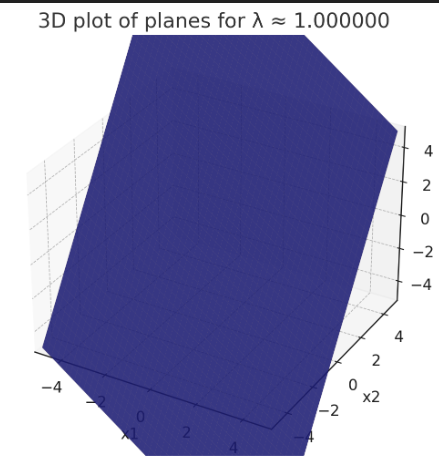
\includegraphics[height=0.4\textheight, keepaspectratio]{5.13.12fig.png}

      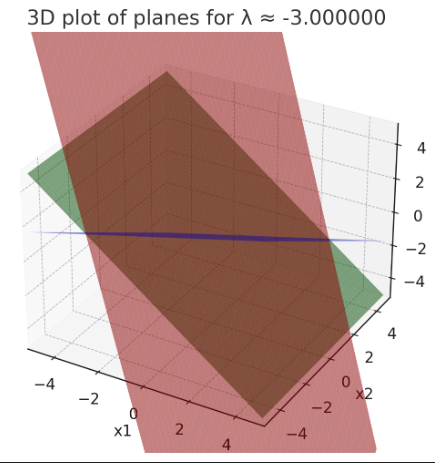
\includegraphics[height=0.4\textheight, keepaspectratio]{5.13.12fig(1).png}
   
    \label{figure_1}
\end{figure}
 
\end{document}